
\documentclass[a4paper, 12pt]{article}

\usepackage{graphicx}

\begin{document}
\title{ARE213 Problem Set \#1A}
\author{Peter Alstone \& Frank Proulx}
\maketitle

\section{Problem \#1}
\subsection{Part A}

Data records are excluded from the dataset based whether the following variables take the noted values \(as found in the data manual\):

\subsection{Part B}
We dropped all rows where any data were missing in that row.  One way that the data cleaning process could be improved would be to only remove records based on the variables of interest (as are determined in subsequent analysis) since missing values in fields that are not eventually used in the analysis do not pose a problem..  This would result in a more iterative approach, however, and increase workload on the researcher.

We used some exploratory analysis to understand if the records that were dropped due to missing data \textit{somewhere} in the record were representative.  First we compared a few simple summary statistics between the "full record" and "partial record" data on variables of interest for this analysis.  These are summarized in Table \ref{tab:compareMissingData}.  Better APGAR scores and lower incidence of smoking may be correlated with having full datasets, which indicates the people who have missing data may bias the sample.  We also used agnostic linear regression to understand the relationship between the presence of full records and three key variables: one-minute apgar (omaps), five-minute apgar (fmaps), and number of cigarettes smoked each day (cigar).  The results summarized in Table \ref{tab:lmMissingData} indicate there is statistical significance in each of the factors (i.e. all three are useful predictors for whether a person has a full data record) but also that the influence of the factors is small.  Figure \ref{fig:cigarFullData} shows the distribution in the number of cigarettes smoked by those with and without full records.  The distribution of values is basically the same (clusters around multiples of five up to 20, or, a "pack a day") between the two datasets.  

Overall, in spite of the bias from removing heavier smokers with lower apgar scores from the data, the overall number removed is relatively small and the size of the bias (indicated by the coefficients in the linear model) is relatively small.  

% Table created by stargazer v.4.0 by Marek Hlavac, Harvard University. E-mail: hlavac at fas.harvard.edu
% Date and time: Thu, Sep 19, 2013 - 16:27:57
\begin{table}[!htbp] \centering 
  \caption{Comparison of data with full records to those with missing data across key variables} 
  \label{tab:compareMissingData} 
\begin{tabular}{@{\extracolsep{5pt}} ccccccc} 
\\[-1.8ex]\hline 
\hline \\[-1.8ex] 
full.record & mean.omaps & sd.omaps & mean.fmaps & sd.fmaps & mean.cigar & sd.cigar \\ 
\hline \\[-1.8ex] 
FALSE & $7.905$ & $1.572$ & $8.880$ & $1.030$ & $3.945$ & $7.422$ \\ 
TRUE & $8.117$ & $1.260$ & $9.009$ & $0.707$ & $1.907$ & $5.297$ \\ 
\hline \\[-1.8ex] 
\normalsize 
\end{tabular} 
\end{table} 


% Table created by stargazer v.4.0 by Marek Hlavac, Harvard University. E-mail: hlavac at fas.harvard.edu
% Date and time: Thu, Sep 19, 2013 - 16:32:14
\begin{table}[!htbp] \centering 
  \caption{Linear model results for predicting whether full records are present based on } 
  \label{tab:lmMissingData} 
\begin{tabular}{@{\extracolsep{5pt}}lc} 
\\[-1.8ex]\hline 
\hline \\[-1.8ex] 
 & \multicolumn{1}{c}{\textit{Dependent variable:}} \\ 
\cline{2-2} 
\\[-1.8ex] & full.record \\ 
\hline \\[-1.8ex] 
 omaps & 0.002$^{***}$ \\ 
  & (0.001) \\ 
  & \\ 
 fmaps & 0.007$^{***}$ \\ 
  & (0.001) \\ 
  & \\ 
 cigar & $-$0.003$^{***}$ \\ 
  & (0.0001) \\ 
  & \\ 
 Constant & 0.882$^{***}$ \\ 
  & (0.007) \\ 
  & \\ 
\hline \\[-1.8ex] 
Observations & 119,384 \\ 
R$^{2}$ & 0.007 \\ 
Adjusted R$^{2}$ & 0.007 \\ 
Residual Std. Error & 0.195 \\ 
F Statistic & 276.305 \\ 
\hline 
\hline \\[-1.8ex] 
\textit{Note:}  & \multicolumn{1}{r}{$^{*}$p$<$0.1; $^{**}$p$<$0.05; $^{***}$p$<$0.01} \\ 
\normalsize 
\end{tabular} 
\end{table}


\begin{figure}[!h] %  figure placement: here, top, bottom, or page
   \centering
   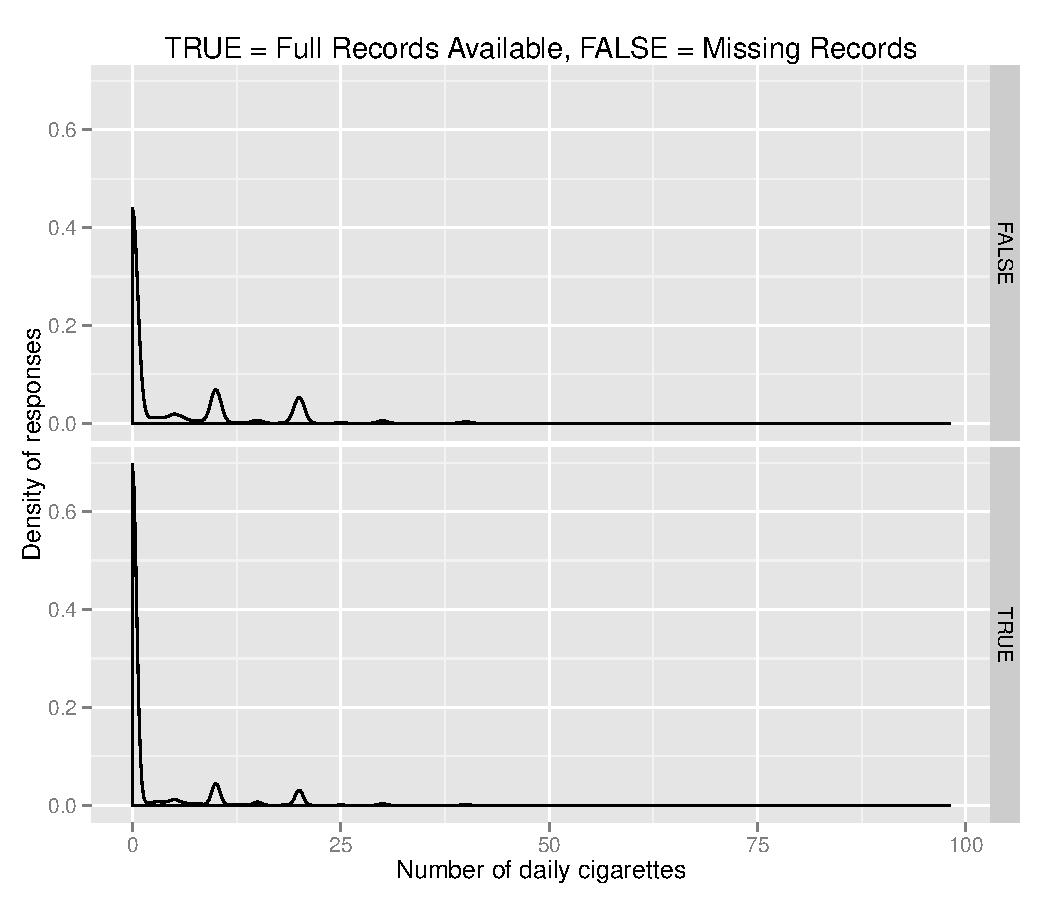
\includegraphics[width=4in]{img/cigar-by-record-type.pdf} 
   \caption{Cigarette use rate by presence of full data record.}
   \label{fig:cigarFullData}
\end{figure}

\subsection{Part C}
The summary table for the remaining data after cleaning is below.
% Code for the summary table from file summarytable.tex starts here...
% latex.default(summarytable) 
%

% Table created by stargazer v.4.5.1 by Marek Hlavac, Harvard University. E-mail: hlavac at fas.harvard.edu
% Date and time: Tue, Sep 17, 2013 - 11:26:06 PM
\begin{table}[!htbp] \centering 
  \caption{Summary of Cleaned Dataset} 
  \label{} 
\begin{tabular}{@{\extracolsep{5pt}}lccccc} 
\\[-1.8ex]\hline 
\hline \\[-1.8ex] 
Statistic & \multicolumn{1}{c}{N} & \multicolumn{1}{c}{Mean} & \multicolumn{1}{c}{St. Dev.} & \multicolumn{1}{c}{Min} & \multicolumn{1}{c}{Max} \\ 
\hline \\[-1.8ex] 
rectype & 114,616 & 1.262 & 0.440 & 1 & 2 \\ 
pldel3 & 114,616 & 1.018 & 0.133 & 1 & 2 \\ 
birattnd & 114,616 & 1.202 & 0.564 & 1 & 5 \\ 
cntocpop & 114,616 & 1.443 & 1.137 & 0 & 3 \\ 
stresfip & 114,616 & 41.743 & 2.167 & 0 & 55 \\ 
dmage & 114,616 & 27.757 & 5.699 & 12 & 49 \\ 
ormoth & 114,616 & 0.091 & 0.522 & 0 & 5 \\ 
mrace3 & 114,616 & 1.259 & 0.657 & 1 & 3 \\ 
dmeduc & 114,616 & 13.211 & 2.272 & 0 & 17 \\ 
dmar & 114,616 & 1.251 & 0.434 & 1 & 2 \\ 
adequacy & 114,616 & 1.297 & 0.546 & 1 & 3 \\ 
nlbnl & 114,616 & 0.967 & 1.148 & 0 & 12 \\ 
dlivord & 114,616 & 1.986 & 1.174 & 1 & 14 \\ 
dtotord & 114,616 & 2.420 & 1.520 & 1 & 24 \\ 
totord9 & 114,616 & 2.407 & 1.458 & 1 & 8 \\ 
monpre & 114,616 & 2.502 & 1.326 & 0 & 9 \\ 
nprevist & 114,616 & 11.152 & 3.524 & 0 & 49 \\ 
disllb & 114,616 & 350.422 & 362.326 & 0 & 777 \\ 
isllb10 & 114,616 & 3.321 & 3.188 & 0 & 9 \\ 
dfage & 114,616 & 30.063 & 6.410 & 13 & 78 \\ 
orfath & 114,616 & 0.095 & 0.531 & 0 & 5 \\ 
dfeduc & 114,616 & 13.277 & 2.326 & 0 & 17 \\ 
birmon & 114,616 & 6.474 & 3.394 & 1 & 12 \\ 
weekday & 114,616 & 4.047 & 1.881 & 1 & 7 \\ 
dgestat & 114,616 & 39.153 & 2.445 & 17 & 47 \\ 
csex & 114,616 & 1.485 & 0.500 & 1 & 2 \\ 
dbrwt & 114,616 & 3,373.295 & 585.168 & 227 & 6,067 \\ 
dplural & 114,616 & 1.028 & 0.174 & 1 & 4 \\ 
omaps & 114,616 & 8.117 & 1.260 & 0 & 10 \\ 
fmaps & 114,616 & 9.009 & 0.707 & 0 & 10 \\ 
clingest & 114,616 & 39.109 & 2.057 & 17 & 44 \\ 
delmeth5 & 114,616 & 1.549 & 1.010 & 1 & 5 \\ 
anemia & 114,616 & 1.990 & 0.099 & 1 & 2 \\ 
cardiac & 114,616 & 1.993 & 0.083 & 1 & 2 \\ 
lung & 114,616 & 1.993 & 0.085 & 1 & 2 \\ 
diabetes & 114,616 & 1.973 & 0.162 & 1 & 2 \\ 
herpes & 114,616 & 1.994 & 0.089 & 1 & 8 \\ 
chyper & 114,616 & 1.992 & 0.087 & 1 & 2 \\ 
phyper & 114,616 & 1.969 & 0.172 & 1 & 2 \\ 
pre4000 & 114,616 & 1.986 & 0.119 & 1 & 2 \\ 
preterm & 114,616 & 1.986 & 0.118 & 1 & 2 \\ 
tobacco & 114,616 & 1.841 & 0.366 & 1 & 2 \\ 
cigar & 114,616 & 1.907 & 5.297 & 0 & 98 \\ 
cigar6 & 114,616 & 0.346 & 0.861 & 0 & 5 \\ 
alcohol & 114,616 & 1.990 & 0.098 & 1 & 2 \\ 
drink & 114,616 & 0.031 & 0.619 & 0 & 91 \\ 
drink5 & 114,616 & 0.020 & 0.230 & 0 & 4 \\ 
wgain & 114,616 & 30.356 & 11.885 & 0 & 98 \\ 
\hline \\[-1.8ex] 
\normalsize 
\end{tabular} 
\end{table} 
\end{document}


%...and ends here.

\section{Problem \#2}
\(a\) The mean differences in 

% latex.default(smoketable) 
%
\begin{table}[!tbp]
\begin{center}
\begin{tabular}{lrrr}
\hline\hline
\multicolumn{1}{l}{smoketable}&\multicolumn{1}{c}{Mean Value (Smokers)}&\multicolumn{1}{c}{Mean Value (Non-Smokers)}&\multicolumn{1}{c}{Mean Difference}\tabularnewline
\hline
1 minute APGAR score&$   8.10275922478923$&$   8.12019719771666$&$1.74379729274321e-02$\tabularnewline
5 munute APGAR score&$   9.00908792291689$&$   9.00922677737416$&$1.38854457262028e-04$\tabularnewline
birthweight&$3171.13916566298030$&$3411.61984431759220$&$2.40480678654612e+02$\tabularnewline
\hline
\end{tabular}
\end{center}
\end{table}



\(b\) The average treatment effect of maternal smoking can be determined by comparing the unadjusted difference in mean birth weight of infants if we have randomized control and treatment groups of mothers.


\pagebreak
\section{Appendix}
R code for problem \#1:
\begin{verbatim}
### This is Frank Proulx's solution to ARE213 PS1a, problem 1
## Data is in the file "ps1.dta"

library(foreign) #this is to read in Stata data
library(Hmisc)
library(psych)
data <- read.dta("ps1.dta")

print(nrow(data))

## Problem 1a: Fix missing values
## The following are the error codes for each of the 15 variables that need fixing:
# cardiac: 9
# lung: 9
# diabetes: 9
# herpes: 9
# chyper: 9
# phyper: 9
# pre4000: 9
# preterm: 9
# tobacco: 9
# cigar: 99
# cigar6: 6
# alcohol: 9
# drink: 99
# drink5: 5
# wgain: 99

data <- subset (data, (cardiac != 9) & (lung != 9) & (diabetes !=9) & (herpes !=9) & (chyper !=9) & (phyper !=9) & (pre4000 !=9) & (preterm !=9) & (tobacco !=9) & (cigar !=99) & (cigar6 !=6) & (alcohol !=9) & (drink !=99) & (drink5 !=5) & (wgain !=99))

print(nrow(data)) #number of records remaining after cleaning

print(describe(data, skew=FALSE, ranges=FALSE))

write.csv(data, file = "ps1dataclean.csv")

#'omaps' and 'fmaps' are the APGAR scores
#'dbrwt' is the birth weight in grams
# 'tobacco' is smoker status (1=yes, 2=no)

smokers <- subset(data, tobacco==1)
nonsmokers <- subset(data, tobacco==2)

smokerstats <- c(mean(smokers$omaps), mean(smokers$fmaps), mean(smokers$dbrwt))
nonsmokerstats <- c(mean(nonsmokers$omaps), mean(nonsmokers$fmaps), mean(nonsmokers$dbrwt))
meandif <- nonsmokerstats - smokerstats

print(smokerstats)
print(nonsmokerstats)
print(meandif)

print(t.test(data$omaps~data$tobacco))
print(t.test(data$fmaps~data$tobacco))
print(t.test(data$dbrwt~data$tobacco))
\end{verbatim}

\end{document}
